\graphicspath{{chapter2/}{manuscript/}}

\chapter{\textbf{\MakeUppercase{  La sensibilité du taux de croissance
des espèces d'arbres au climat et la compétition dans l'ensemble de leur
aire de répartition}}}

\section{Résumé de l'article et contribution}

Les modèles d'aire de répartition basés sur les taux démographiques sont
conçus pour utiliser la variabilité individuelle afin de prédire le taux
de croissance de la population. Ces modèles offrent une approche plus
mécaniste pour évaluer la distribution des espèces que les modèles
phénoménologiques. Malgré le grand nombre de modèles forestiers adoptant
cette approche pour explorer l'influence du climat et de la compétition
sur le taux de croissance de la population des espèces arboricoles, la
corrélation entre la performance des espèces et leur distribution est
souvent faible. Il reste à comprendre si cette faible corrélation entre
la performance des espèces et leurs distributions découle des
limitations des modèles utilisés ou si le climat et la compétition sont
de mauvais prédicteurs pour la distribution des espèces.\\

Dans ce chapitre, nous avons développé un Modèle de Projection Intégrale
pour évaluer l'impact du climat et de la compétition sur chacun des
composants démographiques de 31 espèces d'arbres de l'est de l'Amérique
du Nord. En utilisant des modèles hiérarchiques non linéaires qui
tiennent compte de l'incertitude des processus, nous avons comblé la
plupart des lacunes des études précédentes.\\

En utilisant des analyses de perturbation, nous avons constaté que taux
de croissance de la population était plus sensible à la température
annuelle moyenne qu'à la compétition conspécifique et hétérospécifique
parmis toutes les espèces. Nous avons aussi examiné comment cette
sensibilité variait à travers la répartition des espèces. L'effet
dominant du climat par rapport à celui de la compétition augmentait
lorsque les espèces approchaient des régions aux températures froides ou
chaudes. De plus, la plupart des espèces présentaient un déclin de la
sensibilité de taux de croissance de la population à la compétition en
allant des régions aux températures froides vers les régions aux
tempratures chaudes. Cependant, la variable la plus influente restait
les conditions locales du site, capturées par les effets aléatoires. Ces
résultats fournissent des informations importantes sur la manière dont
les espèces peuvent répondre aux conditions associées aux changements
climatiques et aux perturbations.\\

Cette étude a été conçu par Dominique Gravel et moi-même. Le modèle a
été développé par Andrew MacDonald et moi-même. Les analyses, les
figures et la première version du manuscrit ont été réalisées par
moi-même. Tous les co-auteurs ont contribué à la révision de ce
manuscrit.\\

\vfill{}
\pagebreak

\begin{center}
\textbf{\MakeUppercase{Sensitivity of tree species performance to
climate and competition changes across their range distribution}} \\
Willian~Vieira, Andrew~MacDonald, Dominique~Gravel
\end{center}

\section{Abstract}

Demographic range models, designed to scale individual variation to
predict population growth rate, offer a more mechanistic approach to
assessing species distribution than phenomenological models. Despite
numerous forest models adopting this approach to explore the influence
of climate and competition on species population growth rate, the
correlation of species performance with their distribution is often
weak. What remains unclear is whether the mismatch between species
performance and distribution arises from modelling limitations or if
climate and competition are poor predictors of species distribution.
Here, we developed an Integral Projection Model to evaluate the impact
of climate and competition on all demographic components of 31 tree
species from eastern North America. By using flexible nonlinear
hierarchical models, we filled most of the gaps in previous studies
while accounting for process uncertainty. Using perturbation analysis,
we found that population growth rate was more sensitive to mean annual
temperature than conspecific and heterospecific competition for all
species. Furthermore, we examined how population growth rate sensitivity
to climate and competition varied across the species range. The
dominance of climate over competition increased as species approached
the cold or hot temperature ranges. Moreover, most species exhibited a
decline in population growth rate sensitivity to competition from the
cold to the hot temperature range. Notably, the most influential
variable remained the local plot conditions captured by the random
effects. Unveiling species-specific sensitivity to climate and
competition provides crucial insights into how species may respond to
emerging conditions resulting from climate change and disturbance
changes.\\

\textbf{Keywords}: Integral Projection Models, Perturbation
analysis, demography performance

\hypertarget{introduction}{%
\section{Introduction}\label{introduction}}

The urge to unravel species distribution processes has increased with
the current global crisis, where 15 to 37\% of species are expected to
face extinction due to climate change \citep{thomas2004}. This urgency
is particularly pertinent for long-lived sessile species like trees,
whose range distribution is likely to fail to follow climate change
\citep{Zhu2012, Sittaro2017}. In an effort to enhance traditional
correlative species distribution models \citep[e.g.~][]{Guisan2000},
theory decomposes species distribution into smaller components to
develop a more mechanistic, process-based approach \citep{Evans2016}.
One such approach is demographic range models, which predicts a species'
distribution based on individual performance determined by growth,
survival, and recruitment rates \citep{Pagel2012}. This approach
operates under the hypothesis that population growth rate (\(\lambda\)),
determined by demographic rates, varies across the environment, with the
species range limit defined by conditions where \(\lambda\) is positive
\citep{maguire1973niche, Holt2009}. By approaching species distribution
from a demographic perspective, we can account for the complexity of
forest dynamics arising from multiple features such as environment and
species interaction \citep[Schurr2012;][]{Svenning2014}.\\

Several studies have attempted to predict species distribution based on
demographic performance of forest trees. The most basic version of these
models uses environment-dependent demographic rates to predict
\(\lambda\) \citep[e.g.~][]{Merow2014, Csergo2017}. However, factors
like competition undeniably influence both demographic rates
\citep{Luo2011, Clark2011, Zhang2015} and population performance
\citep{Scherrer2020, LeSquin2021} in forest trees. This realized version
of the niche \citep{Hutchinson1957} may explain why North American
forest trees often do not occur within their climatically suitable range
\citep{BoucherLalonde2012, Talluto2017}.\\

An increasing body of evidence conflicts with theoretical expectations
by observing weak correlations between the demographic performance of
trees and their distribution
\citep{McGill2012, Thuiller2014, Csergo2017, bohner2020, LeSquin2021, Midolo2021, Guyennon2023}.
This mismatch is often attributed to the oversight of processes beyond
climate and competition. For instance, habitat availability coupled with
dispersal limitations can restrict a species' distribution even in
locations where performance is positive \citep{Pulliam2000}. However,
the precision of methods used to quantify demographic performance is
rarely challenged, perhaps in part because each attempt employs a
different approach. Some studies assess performance based solely on one
of the growth, survival, or recruitment rates
\citep{McGill2012, bohner2020}. When demographic rates are integrated
into population models, specific components, such as recruitment, are
often overlooked due to data limitations
\citep{Kunstler2021, LeSquin2021}. Moreover, some studies do not account
for density dependence \citep{Csergo2017, Ohse2023}, and when they do,
they rarely differentiate between conspecific and heterospecific
competition \citep{bohner2020, LeSquin2021}. Finally, despite the need
to embrace model and data uncertainty \citep{MilnerGulland2017a}, most
of these studies assessed performance under average covariate conditions
and pointwise estimations, neglecting the associated uncertainty of the
estimates.\\

Rather than asking whether demographic performance correlates with
distribution, a more fruitful question may be how climate and
competition influence demographic performance. Indeed, we still miss a
comprehensive partitioning of the sensitivity of forest dynamics to
local and biogeographical drivers of performance \citep{Ohse2023}. For
instance, \citet{Clark2011} found that annual growth rate is more
sensitive to competition, while fecundity is more sensitive to climate.
In contrast, \citet{CopenhaverParry2016} found that growth was more
sensitive to climate than competition. These studies provide crucial
insights into how forest trees will respond to climate change and forest
management, supporting conservation planning. However, they only assess
the importance of climate and competition on single demographic
components, lacking a complete picture of population dynamics. This is
especially critical if species are susceptible to variation in
sensitivity to climate and competition across life history stages
\citep{Russell2012, Ettinger2013}. Furthermore, the sensitivity of
\(\lambda\) to climate and competition may depend on the species range
position, such as climate being relatively more important in abiotic
stressful conditions and competition being more critical when climate is
benign \citep{Louthan2015}. Nevertheless, such information is still
lacking for trees \citep{Ohse2023}.\\

Here, we evaluate how climate and competition affect the demography and
population growth rate of the 31 most abundant forest tree species
across Eastern North America. We leverage the complete (26 - 53°)
latitudinal coverage of forest inventories across the US and Canada to
capture the entire range of these species. Specifically, we model each
of the growth, survival, and recruitment vital rates as a function of
mean annual temperature and precipitation, as well as conspecific and
heterospecific basal area density, serving as a proxy for competition
for light. We fit these demographic models with a flexible, non-linear
hierarchical Bayesian model. The non-linear approach captures both the
complexity of trees' demographic rates and the multiple-effect forms of
climate and competition. Furhtermore, the hierarchical Bayesian approach
allows one to account for model uncertainty at different organizational
scales. These demographic rate models are then incorporated into a
size-structured Integral Projection Model (IPM) to quantify the
\(\lambda\) of each species under climate and competition effects.\\

Our primary goal is to use the fitted IPM to compute the sensitivity of
each species' \(\lambda\) to climate and competition across their range.
Employing perturbation analysis, we quantify the relative contribution
of each covariate to changes in \(\lambda\) \citep{Caswell2000}.
Precisely, we assess the species sensitivity of an observed \(\lambda\)
for each plot-year combination based on their specific climate and
competition conditions. This approach enables an evaluation of the
overall sensitivity of \(\lambda\) to a covariate while considering the
inherent variability of the covariate experienced by the species. For
instance, a species may exhibit high sensitivity to temperature, but if
most of its distribution is observed under optimal temperature
conditions, the average sensitivity of the species will be low.\\

Lastly, expanding on previours findings indicating the inability of
North American trees to both expand their cold range and contract their
hot range under climate change \citep{Talluto2017}, we ask if
sensitivity to climate and competition changes across the species' cold
and hot ranges. Furthermore, we explore whether the relative sensitivity
between climate and competition changes across the species' distribution
range. Our integrative approach allows us to assess the relative effects
of climate and competition from demographic rates up to the population
growth rate while accounting for model uncertainties and stand
structure, revealing essential insights into understanding the response
of forest trees to climate change, management practices, and
conservation efforts.\\

\hypertarget{methods}{%
\section{Methods}\label{methods}}

\hypertarget{forest-inventory-and-climate-data}{%
\subsection{Forest inventory and climate
data}\label{forest-inventory-and-climate-data}}

We used two open inventory datasets from eastern North America: the
Forest Inventory and Analysis (FIA) dataset in the United States
\citep{OConnell2007} and the Forest Inventory of Québec
\citep{Naturelles2016}. At the plot level, we focused on plots sampled
at least twice, excluding those that had undergone harvesting to
concentrate solely on natural dynamics. Specifically, we selected
surveys conducted for the FIA dataset using the modern standardized
methodology implemented since 1999. After applying these filters, our
final dataset encompassed nearly 26,000 plots spanning a latitude range
from 26° to 53° (Figure \ref{fig:figsupp1_ch2}). Each plot within the dataset was measured
between 1970 and 2021, with observation frequencies ranging from 2 to 7
times and an average of 3 measurements per plot. The time intervals
between measurements varied from 1 to 40 years, with a median interval
of 7 years (Figure \ref{fig:figsupp1_ch2}).\\

These datasets provide individual-level information on the diameter at
breast height (DBH) and the status (dead or alive) of more than 200
species. From this pool, we selected the 31 most abundant species (Table
\ref{fig:par_var_ch2}). This selection comprises 9 conifer species and 22 hardwood species.
We ensured an even distribution of species across the shade tolerance
axis, with three species classified as very intolerant, nine as
intolerant, eight as intermediate, eight as tolerant, and five as very
tolerant \citep{burns1990silvics}.\\

For the competition metric, we use asymmetric competition for light,
meaning that each individual is affected only by neighbour individuals
of larger size. We quantified asymmetric competition for light for a
focal individual in a given plot by summing the total basal area of all
individuals larger than the focal one, herein BAL. We further split BAL
into the total density of conspecific and heterospecific individuals.
For the climate variable, we obtained the 19 bioclimatic variables with
a 10 \(km^2\) (300 arcsec) resolution grid, covering the period from
1970 to 2018. These climate variables were modeled using the ANUSPLIN
interpolation method \citep{McKenney2011}. We used each plot's latitude
and longitude coordinates to extract the mean annual temperature (MAT)
and mean annual precipitation (MAP). In cases where plots did not fall
within a valid pixel of the climate variable grid, we interpolated the
climate condition using the eight neighboring cells. Due to the
transitional nature of the dataset, we considered both the average and
standard deviation of MAT and MAP over the years within each time
interval.\\

\hypertarget{model}{%
\subsection{Model}\label{model}}

We evaluated the population growth rates of the 31 forest species using
an Integral Projection Model (IPM). An IPM is a mathematical tool used
to represent the dynamics of structured populations and communities. It
distinguishes itself from traditional population models with the
representation of a continuous trait in discrete time
\citep{Easterling2000}. This is especially relevant for trees due to the
considerable variability in demographic rates depending on individual
size \citep{kohyama1992}. Specifically, the IPM consists of a set of
functions predicting the transition of a distribution of individual
traits from time \(t\) to time \(t+1\):\\

\begin{equation}
n(z', t + 1) = \int_{L}^{U} \, K(z', z, \theta)\, n(z, t)\, \mathrm{d}z
\label{eq:ipm}\end{equation}\\

The continuous trait \(z\) at time \(t\) represents the DBH, bouded
between the lower (\(L\)) and upper (\(U\)) values, and \(n(z, t)\)
characterizes the continuous DBH distribution for a population. The
probability of the population distribution size from \(n(z, t)\) to
\(n(z', t+1)\) is governed by the kernel \(K\) and the species-specific
parameters \(\theta\). The kernel \(K\), a continuous version of the
discretized projection Matrix in structured population models, is
composed of three sub-models:\\

\begin{equation}
K(z', z, \theta) = [Growth(z', z, \theta) \times Survival(z, \theta)] + Recruitment(z, \theta)
\label{eq:kernel}\end{equation}\\

The growth function describes how individual trees increase in size,
while the survival function determines the probability of staying alive
throughout the next time step. The recruitment model describes the
number of individuals ingressing the population. Below, we describe the
basic (intercept) version of these models, followed by the inclusion of
each climate and competition covariate.\\

\hypertarget{demographic-rates}{%
\subsubsection{Demographic rates}\label{demographic-rates}}

\textbf{Growth} - the size in DBH of an individual at time
\(t + \Delta t\) after growing from time \(t\) is determined by:\\

\begin{equation}
  dbh_{i,t + \Delta t} \sim N(\mu_{i, t+\Delta t}, \sigma)
\label{eq:VBlik}\end{equation}\\

We used the von Bertalanffy growth equation to describe the annual
growth rate in DBH of an individual \(i\) \citep{von1957quantitative}.
The average size at time \(t+\Delta t\) from the initial size
\(dbh_{i, t}\) of an individual at time \(t\) is given by:\\

\begin{equation}
  \mu_{i, t+\Delta t} = dbh_{i,t}  \times e^{-\Gamma \Delta t} + \zeta_{\infty} (1- e^{-\Gamma \Delta t})
\label{eq:VBmodel}\end{equation}\\

Where \(\Delta t\) is the time interval between the initial and final
size measurements and \(\Gamma\) represents a dimensionless growth rate
coefficient. \(\zeta_{\infty}\) denotes the asymptotic size, which is
the location at which growth approximates to zero. The rationale behind
this model is that the growth rate exponentially decreases with size,
converging to zero as size approaches \(\zeta_{\infty}\). This
assumption is particularly valuable in the context of the IPM, as it
prevents eviction --- where individuals are projected beyond the limits
of the size distribution (\([L, U]\)) defined by the Kernel.\\

\textbf{Survival} - The chance of a mortality event (\(M\)) for an
individual \(i\) within the time interval between \(t\) and
\(t+\Delta t\) is modeled as a Bernoulli distribution:\\

\begin{equation}
M_i \sim Bernoulli(p_i)
\label{eq:survL}\end{equation}\\

Here, \(M_i\) represents the individual's status (alive/dead) and
\(p_i\) the mortality probability of the individual \(i\). The mortality
probability is calculated based on the annual survival rate (\(\psi\))
and the time interval between census (\(\Delta t\)):\\

\begin{equation}
p_i = 1 - \psi^{\Delta t}
\label{eq:survP}\end{equation}\\

The model assumes that the survival probability (\(1 - p_i\)) increases
with the longevity parameter \(\psi\), but is compensated exponentially
with the increase in time \(\Delta t\).\\

\textbf{Recruitment} - We combined data from the U.S. and Quebec forest
inventories to obtain a broader range of climatic conditions. However,
these inventories have inconsistent protocols for recording seedlings,
saplings, and juveniles. Most of all, they have different size
thresholds for individual-based measurements. Therefore, we quantified
the recruitment rate (\(I\)) as the ingrowth of new individuals into the
adult population, defined as those with a DBH exceeding 12.7 cm. The
quantity \(I\) encompasses the processes of fecundity, dispersal,
growth, and survival up to reaching the size threshold. Similar to
growth and survival, the count of ingrowth individuals (\(I\)) reaching
the 12.7 cm size threshold depends on the time interval between
measurements. We introduce two parameters to control the potential
number of recruited individuals: \(\phi\), determining the annual
ingrowth rate per square meter, and \(\rho\), denoting the annual
survival probability of each ingrowth individual:\\

\begin{equation}
  I \sim Poisson(~\phi \times A \times \frac{1 - \rho^{\Delta t}}{1-\rho}~)
\label{eq:rec}\end{equation}\\

Where \(A\) represents the area of the plot in square meters. The model
assumes that new individuals enter the population annually at a rate of
\(\phi\), and their likelihood of surviving until the subsequent
measurement (\(\rho\)) declines over time. Note that \(\rho\) in
Equation \ref{eq:rec} is not associated with Equation \ref{eq:survP}
determining the survival of the adults. Instead, \(\rho\) is estimated
from the data of individuals arriving in the population. Once an
individual is recruited into the population, a submodel determines its
initial size \(z_I\), increasing linearly with time:\\

\begin{equation}
  z_{I} \sim TNormal(\Omega + \beta \Delta t,~\sigma, ~ \alpha, ~ \beta)
\label{eq:recSize}\end{equation}\\

The \(TNormal\) is a truncated distribution with lower and upper limits
determined by the \(\alpha\) and \(\beta\) parameters, respectively. We
set \(\alpha\) to 12.7 cm, aligning it with the ingrowth threshold,
while \(\beta\) is set to infinity to allow for an unbounded upper
limit.\\

\hypertarget{covariates}{%
\subsubsection{Covariates}\label{covariates}}

\textbf{Random effects} - We introduced plot-level random effects in
each of the growth, survival, and recruitment demographic component to
account for shared variance between the individuals within the same
plot. For a demographic component with an average intercept
\(\overline{I}\), an offset value (\(\alpha\)) is drawn for each plot
\(j\) from a normal distribution with a mean of zero and variance
\(\sigma\):\\

\begin{equation}
\begin{split}
&\alpha_{j} \sim N(0, \sigma) \\[2pt]
&I_j = \overline{I} + \alpha_j
\end{split}
\label{eq:randomEffect}\end{equation}\\

Where \(\sigma\) represents the variance among all plots \(j\) and \(I\)
can take one of three forms: \(\Gamma\) for growth, \(\psi\) for
survival, and \(\phi\) for the recruitment model.\\

\textbf{Competition} - We used basal area of larger individuals (BAL;
asymmetric competition) instead of total basal area (BA; symmetric
competition), assuming that competition for light is the primary
competitive factor driving forest dynamics \citep{Pacala1996a}.
Therefore, each of the growth (\(\Gamma\)), longevity (\(\psi\)), and
recruitment survival (\(\rho\)) parameters decreases exponentially with
BAL. Take \(I\) as one of the three parameters, the effect of BAL on
\(I\) is driven by two parameters describing the conspecific (\(\beta\))
and heterospecific (\(\theta\)) competition:\\

\begin{equation}
  I + \beta (BAL_{cons} + \theta \times BAL_{het})
\label{eq:compEffect}\end{equation}\\

When \(\theta < 1\), conspecific competition is stronger than
heterospecific competition. Conversely, heterospecific competition
prevails when \(\theta > 1\), and when \(\theta = 1\), there is no
distinction between conspecific and heterospecific competition. Note
that \(\beta\) is also unbounded, allowing it to converge towards
negative (indicating competition) or positive (indicating facilitation)
values. Furthermore, we fixed \(\theta = 1\) for the recruitment
(\(I = \rho\)) due to model convergence issues. The recruitment model
also accounts for the conspecific density dependence effect on the
annual ingrowth rate (\(\phi\)). Specifically, \(\phi\) increases with
\(BAL_{cons}\) as a positive effect of seed source up to reach the
optimal density of recruitment, \(\delta\), where it then decreases with
more conspecific density due to competition at a rate proportional to
\(\sigma\):\\

\begin{equation}
  \phi + \left(\frac{BAL_{cons} - \delta}{\sigma}\right)^2
\label{eq:compingrowth}\end{equation}\\

\textbf{Climate} - We selected mean annual temperature (MAT) and mean
annual precipitation (MAP) bioclimatic variables as they are widely used
in species distribution modeling and were previously found relevant to
model demography of these species \citep{LeSquin2021}. Each demographic
component \(I\), representing either \(\Gamma\) for growth, \(\psi\) for
longevity, or \(\phi\) for ingrowth, varies as a bell-shaped curve
determined by an optimal climate condition (\(\xi\)) and a climate
breadth parameter (\(\sigma\)):\\

\begin{equation}
  I + \left(\frac{MAT - \xi_{MAT}}{\sigma_{MAT}}\right)^2 + \left(\frac{MAP - \xi_{MAP}}{\sigma_{MAP}}\right)^2
\label{eq:compEffect}\end{equation}\\

The climate breadth parameter (\(\sigma\)) influences the strength of
the specific climate variable's effect on each demographic component.
This unimodal function is flexible, assuming various shapes, such as
bell, quasi-linear, or flat shapes. However, this flexibility introduces
the possibility of parameter degeneracy or redundancy, where different
combinations of parameter values yield similar outcomes. To address this
issue, we constrained the optimal climate condition parameter (\(\xi\))
within the observed climate range for the species, assuming that the
optimal climate condition falls within our observed data range.\\

\hypertarget{model-fit-and-validation}{%
\subsubsection{Model fit and
validation}\label{model-fit-and-validation}}

We fitted each of the growth, survival, and recruitment models
separately for each species, using the Hamiltonian Monte Carlo (HMC)
algorithm implemented in the Stan software \citep[version
2.30.1][]{stan2022stan} with the \texttt{cmdstandr} R package interface
\citep[version 0.5.3][]{cmdstanr}. We conducted 2000 iterations for the
warm-up and 2000 iterations for the sampling phase for each of the four
chains, resulting in 8000 posterior samples (excluding the warm-up).
However, we kept only the last 1000 iterations of the sampling phase to
save computation time and storage space, resulting in 4000 posterior
samples. We build and fit each demographic component incrementally, from
a simple intercept, and gradually incorporate plot random effects,
competition, and climate covariates. Recall that our goal is not to have
the most complex model to achieve the highest predictive metric but to
make inferences \citep{Tredennick2021}. We focus on assessing the
relative effects of climate and competition while controlling for other
influential factors. Therefore, our modeling approach is guided by
biological mechanisms, which tend to provide more robust extrapolation
\citep{Briscoe2019} rather than being solely dictated by specific
statistical metrics. Nevertheless, we checked if increasing model
complexity with new covariates does not result in worse performance
using complementary metrics such as mean squared error (MSE), pseudo
\(R^2\) \citep{Gelman2019}, and Leave-One-Out Cross-Validation (LOO-CV).
Detailed discussions regarding model fit, diagnostics, and model
comparison can be found in supplementary material 1.\\

With the fitted demographic components, we constructed the Kernel \(K\)
of the IPM following Equation \ref{eq:kernel}. We employed the mid-point
rule to perform the discrete-form integration of the continuous \(K\)
\citep{Ellner2016}. This involved discretizing the projection kernel
\(K\) using bins of 0.1 cm, which are considered appropriate for
obtaining unbiased estimates \citep{zuidema2010integral}. Finally, we
computed the asymptotic population growth rate (\(\lambda\)) using the
leading eigenvalue of the discretized matrix \(K\).\\

\hypertarget{perturbation-analysis}{%
\subsection{Perturbation analysis}\label{perturbation-analysis}}

We use perturbation analysis to assess the sensitivity of \(\lambda\) to
competition and climate conditions \citep{Caswell2000}. We define
sensitivity as the partial derivative of \(\lambda\) with respect to a
covariate \(X\), which can take the form of either conspecific or
heterospecific density dependence competition, or temperature or
precipitation climate conditions. In practice, we quantify sensitivity
by slightly increasing each covariate value \(X_j\) to \(X_j^{'}\) and
computing the change in \(\lambda\) following the right-hand part of
Equation \ref{eq:sens}:\\

\begin{equation}
    \frac{\partial \lambda_{ij}}{\partial X_j} \bigg\rvert_{K_{ij}} \approx \frac{\Delta \lambda_{ij}}{\Delta X_j} = \frac{|f(X_j^{'}) - f(X_j)|}{X_j^{'} - X_j}
\label{eq:sens}\end{equation}\\

Sensitivity is evaluated separately for each species \(i\) and is
conditional on the specific climate and competition conditions observed
for the plot \(j\), along with the Kernel \(K_{ij}\) parameters. We set
the perturbation size to a 1\% increase in the normalized scale for each
covariate. For instance, a 1\% increase translates to a rise of 0.3°C
for Mean Annual Temperature (MAT) and 26 mm for Mean Annual
Precipitation (MAP). Because the competition metric is computed at the
individual level, the perturbation was applied to each individual, where
a 1\% increase corresponds approximately to a rise of 1.2 cm in dbh. As
we were interested in the absolute difference, the resulting sensitivity
value ranges between 0 and infinity, with lower values indicating a
lower sensitivity of \(\lambda\) to the specific covariate. We computed
the log ratio between competition and climate (\(CCR\)) sensitivities to
discern their relative effects as follows:\\

\begin{equation}
\begin{split}
&S_{comp, ij} = \frac{\partial \lambda_{ij}}{\partial BA_{cons, i}} + \frac{\partial \lambda_{ij}}{\partial BA_{het, i}} \\[2pt]
&S_{clim, ij} = \frac{\partial \lambda_{ij}}{\partial MAT_{i}} + \frac{\partial \lambda_{ij}}{\partial MAP_{i}} \\[2pt]
&CCR_{ij} = \text{ln} \frac{S_{comp, ij}}{S_{clim, ij}}
\end{split}
\label{eq:CCR}\end{equation}\\

Here, \(S\) represents the total sensitivity of species \(i\) to
competition or climate for a given plot \(j\). Negative \(CCR\) values
indicate higher sensitivity of \(\lambda\) to climate, while positive
values indicate the opposite.\\

When averaging \(S_{X,i}\) across \(j\), this metric reflects the
sensitivity of \(\lambda_i\) to \(X\), which is conditional upon the
probability distribution of the covariate \(X\). We categorized each
plot into cold, center, or hot conditions along the MAT axis for every
species. Plots were labeled as cold (or hot) if the average MAT fell
below (above) the 10\% (90\%) probability distribution, with all
intermediate plots considered center plots. Thus, sensitivity to a
covariate in the cold range of the species signifies the average
sensitivity among all plots classified as cold. It is important to note
that this classification is also conditional on the probability
distribution of observed MAT within the species.\\

The code to fit each demographic component is available in the
\href{https://github.com/willvieira/TreesDemography}{\texttt{TreesDemography}}
GitHub repository. The code for the IPM model and the respective
sensitivity analysis is available in the
\href{https://github.com/willvieira/forest-IPM/tree/master/simulations/covariates_perturbation}{\texttt{forest-IPM}}
GitHub repository.\\

\hypertarget{results}{%
\section{Results}\label{results}}

\hypertarget{model-validation}{%
\subsection{Model validation}\label{model-validation}}

All species-specific demographic components demonstrated convergence
with \(\hat{R} <1.05\) and low to no divergent iterations. In comparing
the simple intercept model with the more complete versions, the LOO-CV
consistently favored the complete model for all three demographic rates,
featuring plot random effects, competition, and climate covariates, over
other competing models (supplementary material 1). The absolute values
of LOO-CV suggested that the growth model gained the most information
from including covariates, followed by recruitment and survival models.
We further validated our model predictions by comparing the parameters
with traits groups such as growth rate classes, maximum observed size,
maximum observed age, shade tolerance, and seed mass
\citep{burns1990silvics, diaz2022}.\\

The growth model intercept comprises two parameters, one determining the
asymptotic size (\(\zeta_{\infty}\)) and the annual growth rate
\(\Gamma\). The \(\zeta_{\infty}\) can be interpreted as the maximum
predicted size of the species, which correlates well across all 31
species with the maximum observed size in the literature
(\(R^2 = 0.31\), Figure \ref{fig:crossGrowthSurv}). Similarly,
\(\Gamma\) among the species exhibited a distribution aligning with the
fast, moderate, and slow-growing traits (Figure \ref{fig:figsupp2_ch2}). In the survival
model, the expected longevity (\(L\)) can be derived from the annual
survival rate ( \(\psi\)) following the equality \(L = e^{\psi}\),
showing a high correlation with the maximum observed age in the
literature (\(R^2 = 0.59\), Figure \ref{fig:crossGrowthSurv}). In the
recruitment model, the log of the annual ingrowth rate (\(\phi\))
reduced linearly with seed mass (Figure \ref{fig:figsupp3_ch2}), capturing the seed
mass-growth rate tradeoff \citep{Reich1998}. Additionally, the annual
survival probability of ingrowth (\(\rho\)) decreased with intolerance
to shade (Figure \ref{fig:figsupp4_ch2}).\\

\hypertarget{fig:crossGrowthSurv}{%
\begin{figure}
\centering
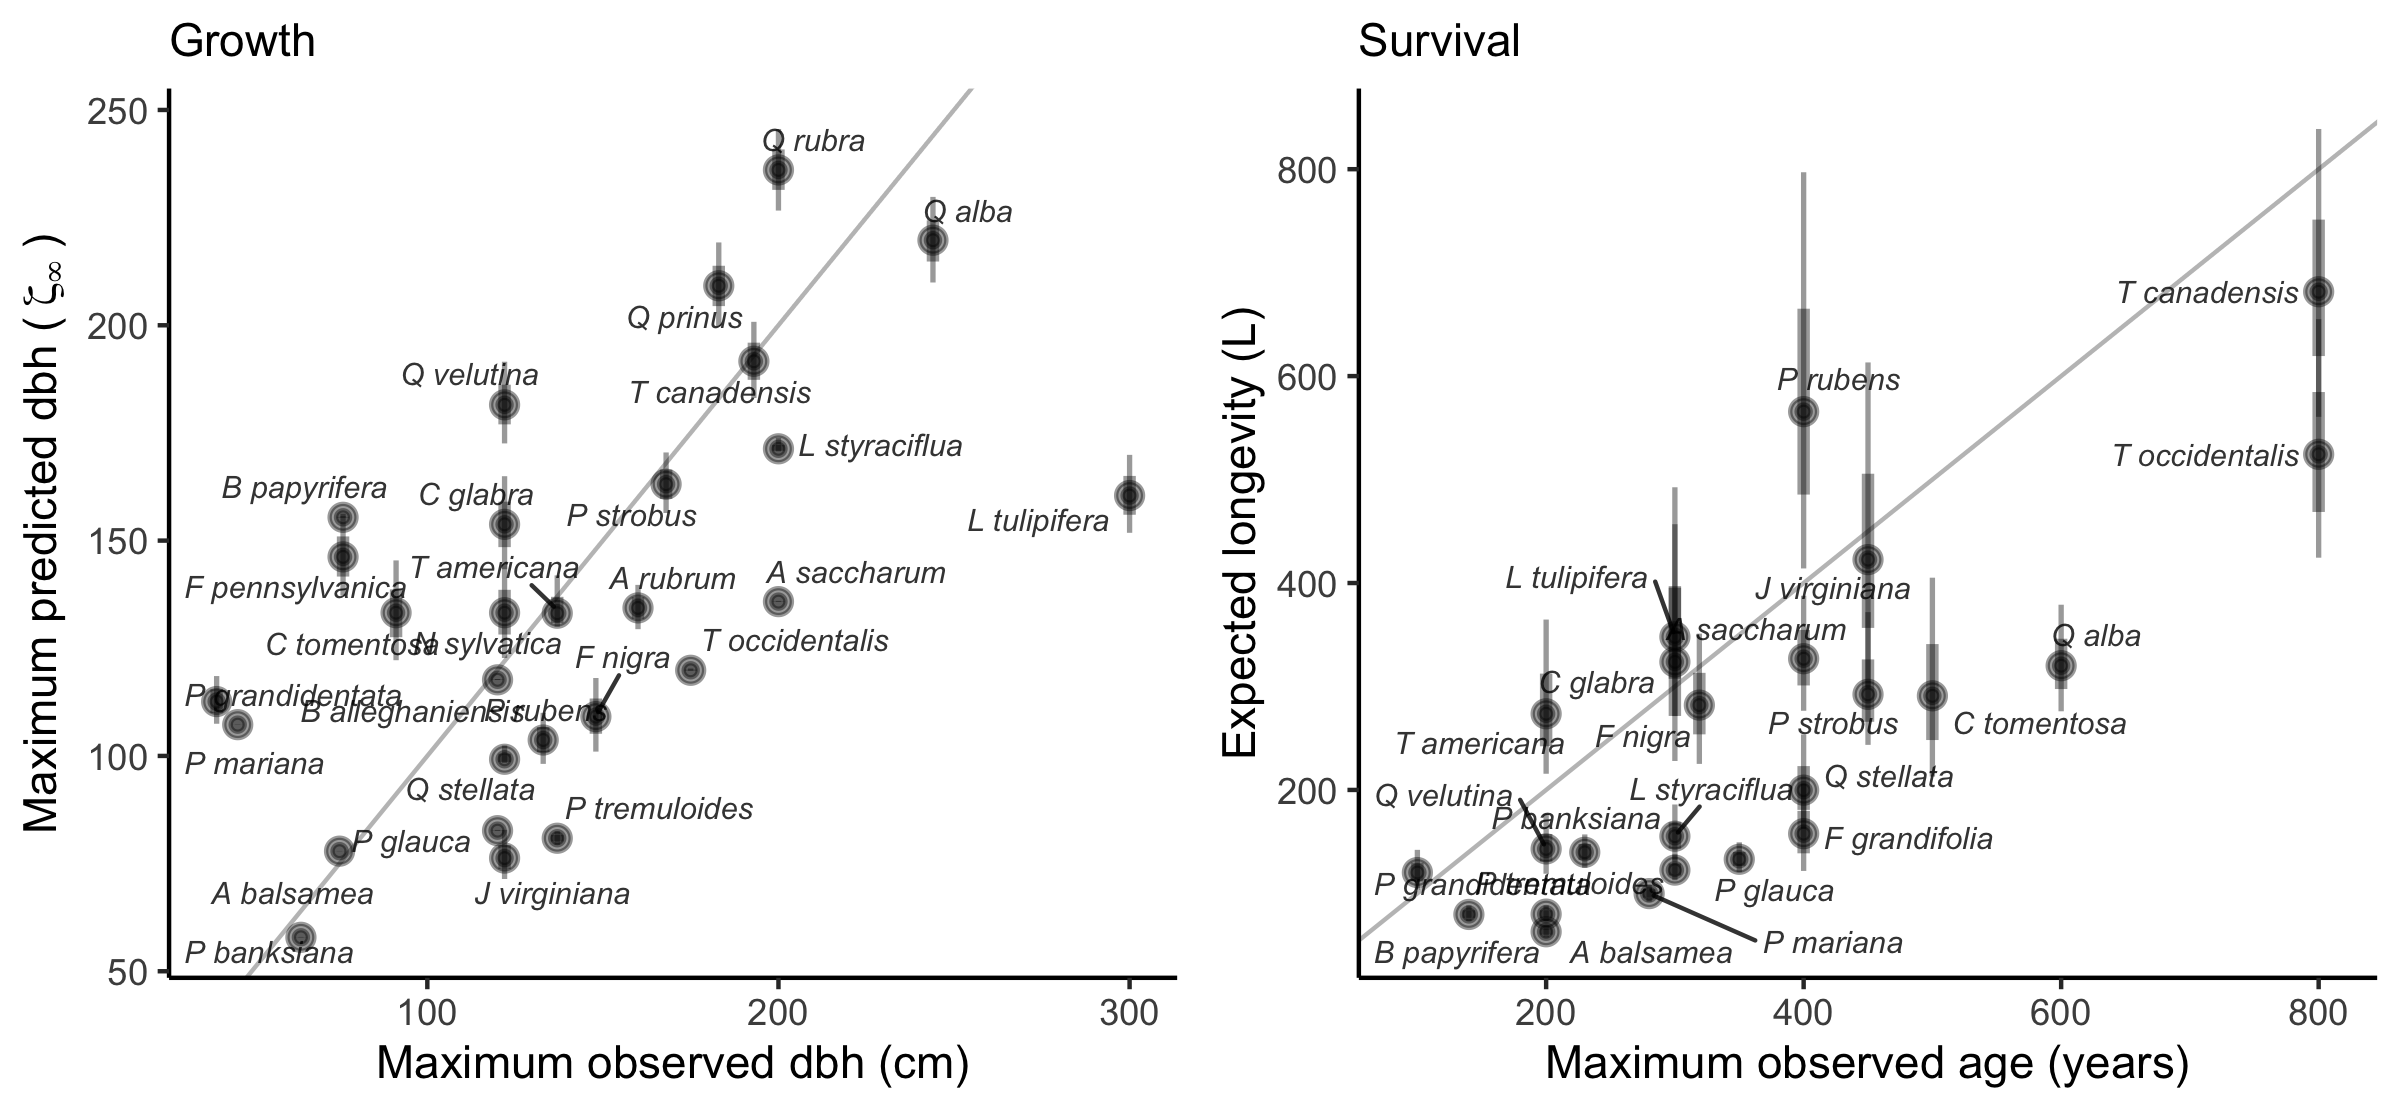
\includegraphics[width=1\textwidth,height=\textheight]{manuscript/figs/crossGrowthSurv.png}
\caption[{Correlation between predicted asymptotic size
(\(\zeta_{\infty}\)) with maximum observed size (left) and predicted
longevity (\(L\)) with maximum observed age for the 31 forest
species.}]{Correlation between predicted asymptotic size
(\(\zeta_{\infty}\)) with maximum observed size (left) and predicted
longevity (\(L\)) with maximum observed age for the 31 forest species.
Maximum observed size and age are obtained from
\citet{burns1990silvics}. The gray line is the identity curve.}
\label{fig:crossGrowthSurv}
\end{figure}
}

Both conspecific and heterospecific competition effects for the growth
and survival models increased with intolerance to shade (Figure
\ref{fig:crossComp}). The stronger competition effect of conspecific
over heterospecific was consistent for almost all species in both growth
and survival models. Only two species for growth and three for survival
among the 31 presented stronger heterospecific competition than
conspecific competition. Moreover, \emph{Fagus grandifolia} and
\emph{Thuja occidentalis} exhibited positive density dependence for the
survival model. For recruitment, the effect of total stand density
increased with shade intolerance among the species (Figure \ref{fig:figsupp5_ch2}).\\

\hypertarget{fig:crossComp}{%
\begin{figure}
\centering
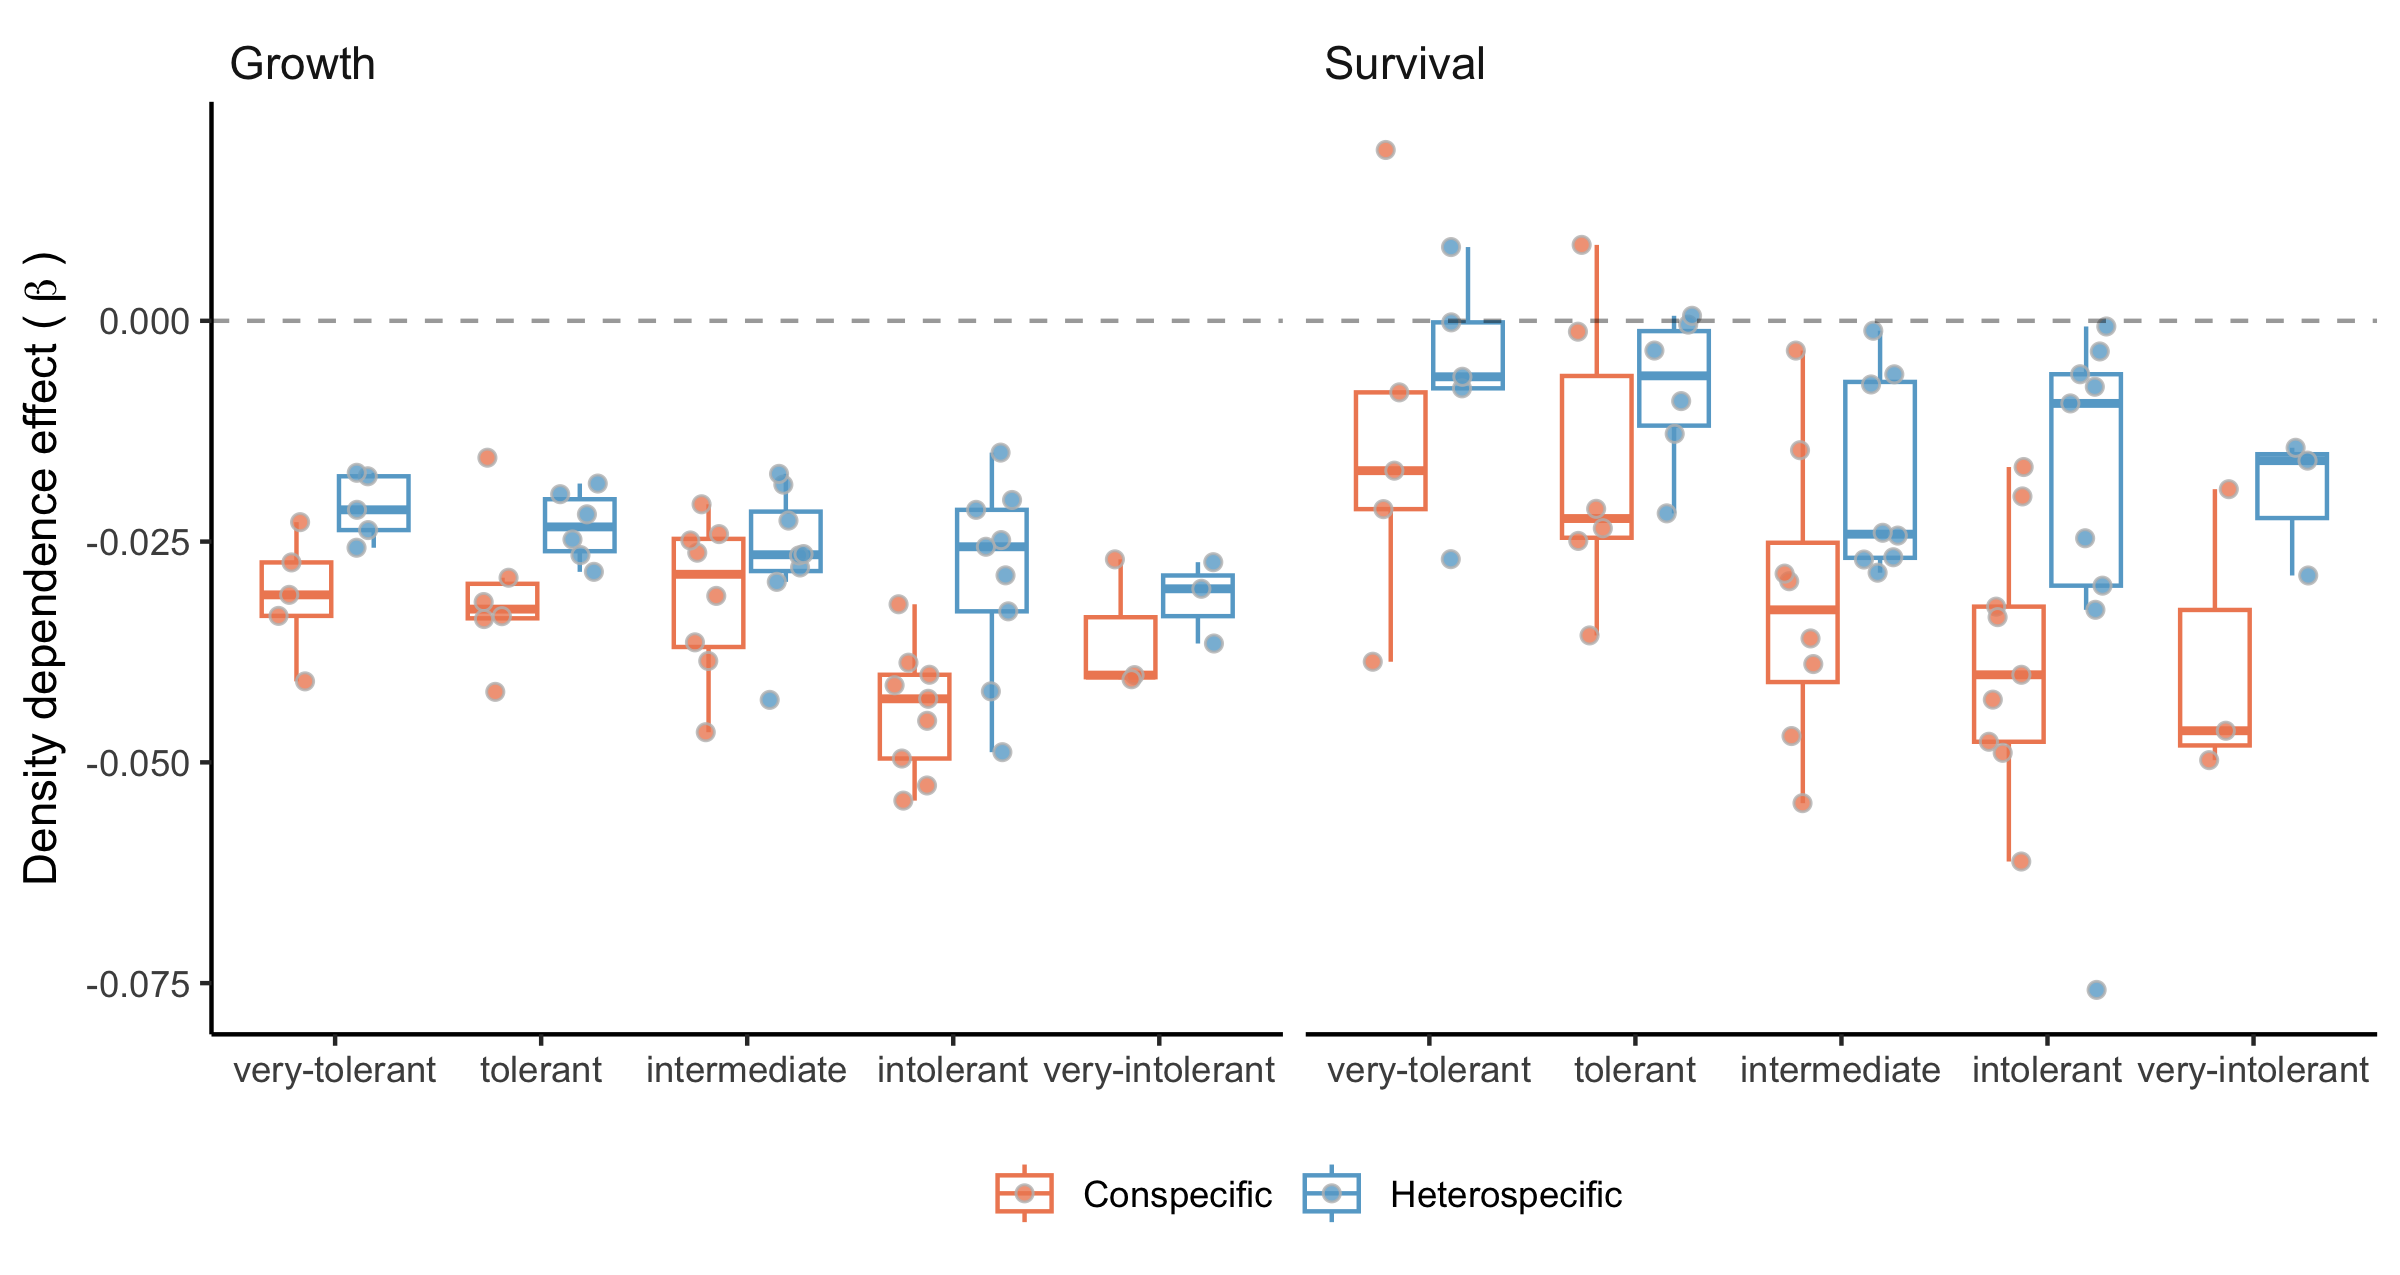
\includegraphics[width=1\textwidth,height=\textheight]{manuscript/figs/crossComp.png}
\caption[{Posterior distribution for the conspecific (red) and
heterospecific (blue) density dependence for each class of shade
tolerance \citep{burns1990silvics}.}]{Posterior distribution for the
conspecific (red) and heterospecific (blue) density dependence for each
class of shade tolerance \citep{burns1990silvics}. The more negative the
\(\beta\), the stronger the competition effect.}
\label{fig:crossComp}
\end{figure}
}

The distribution of optimal MAT (\(\xi_{MAT}\)) and MAP (\(\xi_{MAP}\))
for the 31 species revealed that the optimal climates for growth,
survival, and recruitment were rarely located at the center of the
species ranges (Figure \ref{fig:figsupp6_ch2} and \ref{fig:figsupp7_ch2}). Furthermore, most species exhibited
some degree of demographic compensation, that is, opposing responses to
the environment between demographic rates \citep{Villellas2015}. Lastly,
the climate breadth (\(\sigma\)) determined how flat or narrow the
performance of species was across MAT and MAP. We found among all
species that climate breadth increased with range size, demonstrating
that species with more range occupancy had larger niche breadths. The
exception was the niche breadth of survival over MAT, showing a weak,
flat correlation.\\

\hypertarget{lambda-sensitivity-to-climate-and-competition}{%
\subsection{\texorpdfstring{\(\lambda\) sensitivity to climate and
competition}{\textbackslash lambda sensitivity to climate and competition}}\label{lambda-sensitivity-to-climate-and-competition}}

We used perturbation analysis to assess the relative contribution of
each covariate to changes in \(\lambda\). Figure \ref{fig:mean_sens}
describes the average sensitivity of each species' population growth
rate to conspecific and heterospecific competition, temperature, and
precipitation. Across all species, \(\lambda\) exhibited higher
sensitivity to temperature, followed by conspecific and heterospecific
competition, while sensitivity to mean annual precipitation was
practically zero. This observation of sensitivity to the covariates was
consistent across all species.\\

\hypertarget{fig:mean_sens}{%
\begin{figure}
\centering
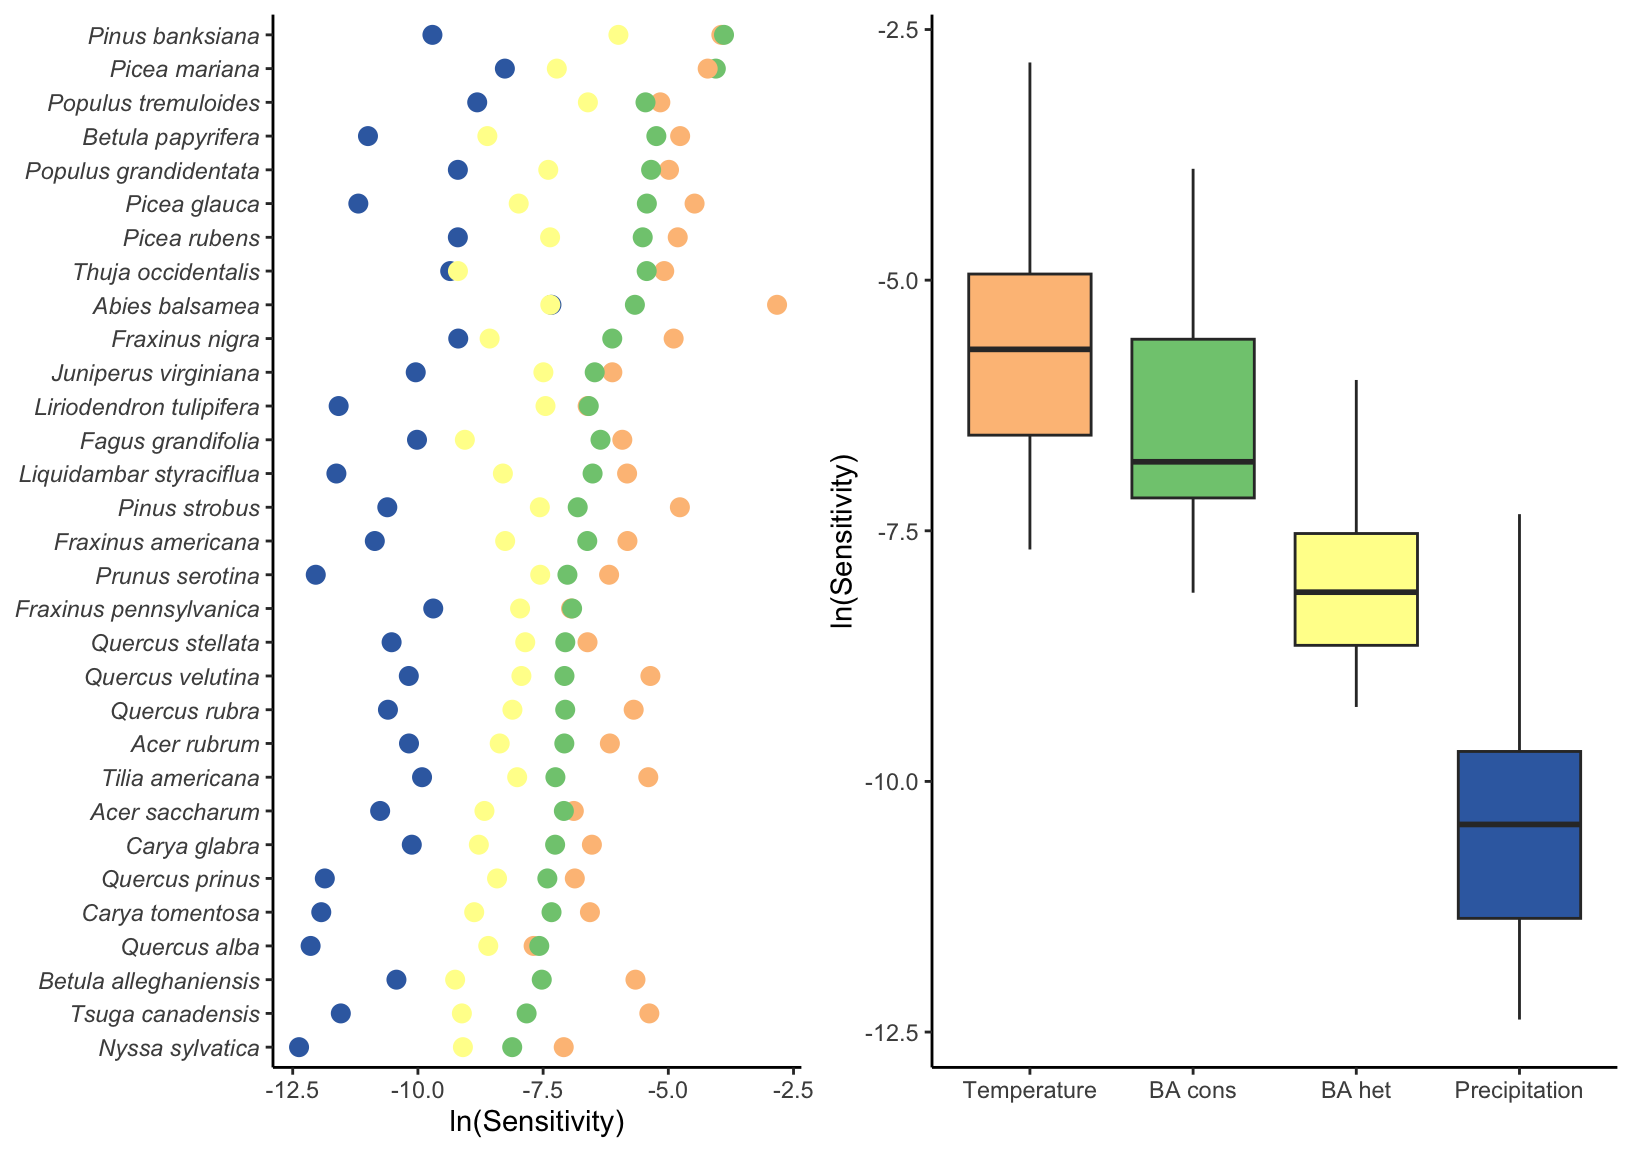
\includegraphics[width=1\textwidth,height=\textheight]{manuscript/figs/fig-ame-1.png}
\caption[{Log sensitivity of species population growth rate to
conspecific competition, heterospecific competition, mean annual
temperature, and mean annual precipitation across all plot-year
observations.}]{Log sensitivity of species population growth rate to
conspecific competition, heterospecific competition, mean annual
temperature, and mean annual precipitation across all plot-year
observations. The smaller the values, the lower the sensitivity to a
covariate.}
\label{fig:mean_sens}
\end{figure}
}

We split plots into different regions to ask for each species if
sensitivity to climate and competition changes between cold and hot
portions of the range (Figure \ref{fig:cold_vs_hot}). We evaluate the
sensitivity of each species' border location according to the average
Mean Annual Temperature (MAT) among all plots of the species' border
group. Species distributed toward colder temperature ranges often
exhibited a decrease in sensitivity to climate from the cold to the hot
border. Conversely, most species in the hot range distribution
demonstrated increased sensitivity to climate at the hot border compared
to the cold. Most species also presented a decreased sensitivity to
competition from the cold to the hot border. The decrease in sensitivity
to competition from the cold to the hot border was more pronounced for
boreal species.\\

\hypertarget{fig:cold_vs_hot}{%
\begin{figure}
\centering
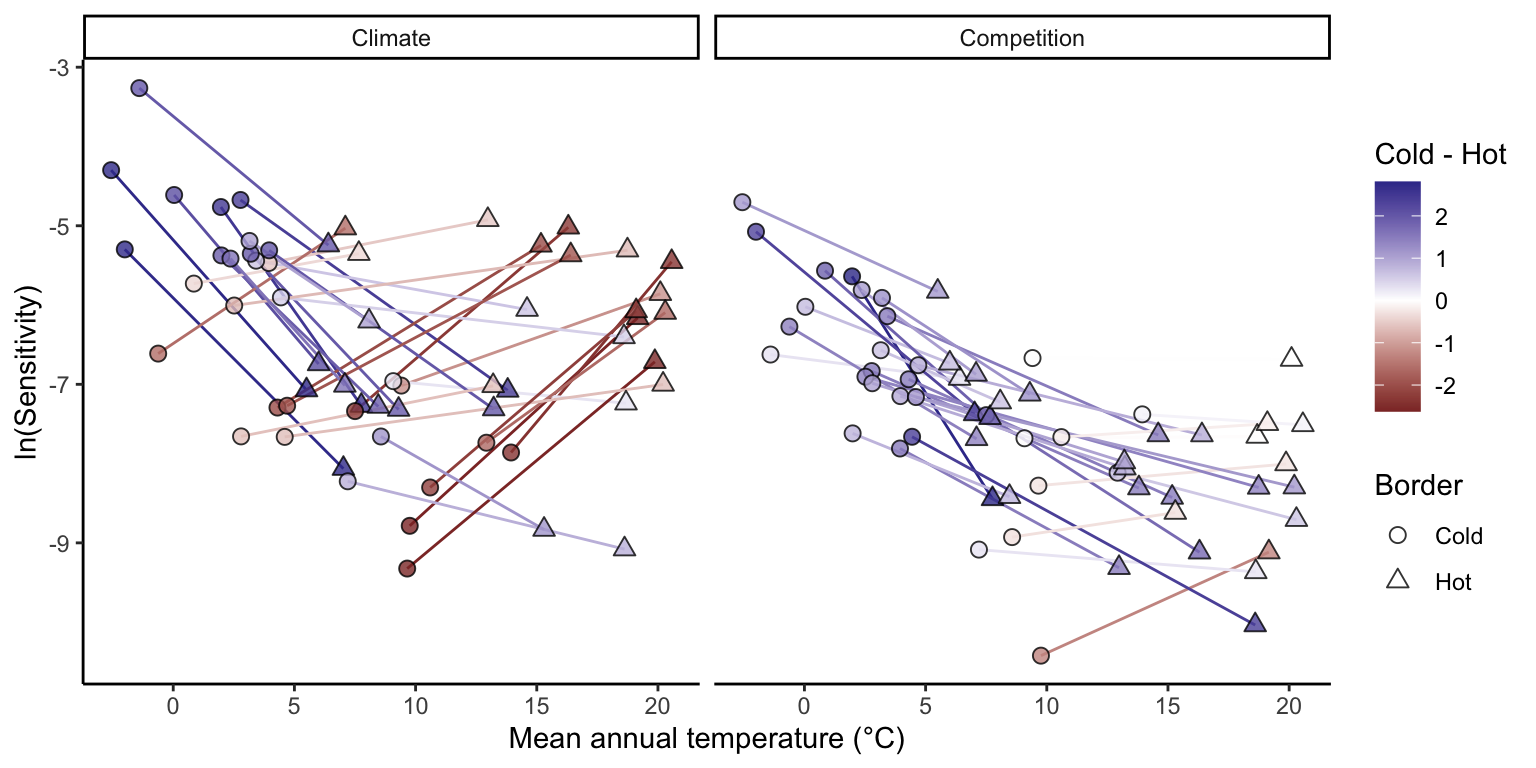
\includegraphics[width=1\textwidth,height=\textheight]{manuscript/figs/fig-hot_vs_cold-1.png}
\caption[{Differences in species population growth rate sensitivity to
climate (left) and competition between the cold and hot range
limits.}]{Differences in species population growth rate sensitivity to
climate (left) and competition between the cold and hot range limits.
Each species is represented by a connected line linking their cold
(circle) and hot (triangle) range positions, colored according to the
difference between the cold and hot sensitivities. Note that uncertainty
in each sensitivity point estimation has been omitted for clarity.}
\label{fig:cold_vs_hot}
\end{figure}
}

We further explore the relative sensitivity between climate and
competition changes across the species' range distribution (Figure
\ref{fig:temp_vs_comp}). \(\lambda\) was more sensitive to climate than
competition for almost all species across the cold, center, and hot
ranges (\(ln(CCR)\) below zero). Across the MAT range distribution, the
relative effect of climate to competition increased toward both the cold
and hot borders of the range. This indicates that species located at the
extremes of the MAT range distribution are even more sensitive to
climate than species at the center. Interestingly, the reason for this
increase is not the same for the cold and hot ranges. In the cold range,
the sensitivity of \(\lambda\) increased for both climate and
competition but was proportionally larger for climate. Conversely, in
the hot range, the relative sensitivity to climate increased due to a
significant decrease in sensitivity to competition.\\

\hypertarget{fig:temp_vs_comp}{%
\begin{figure}
\centering
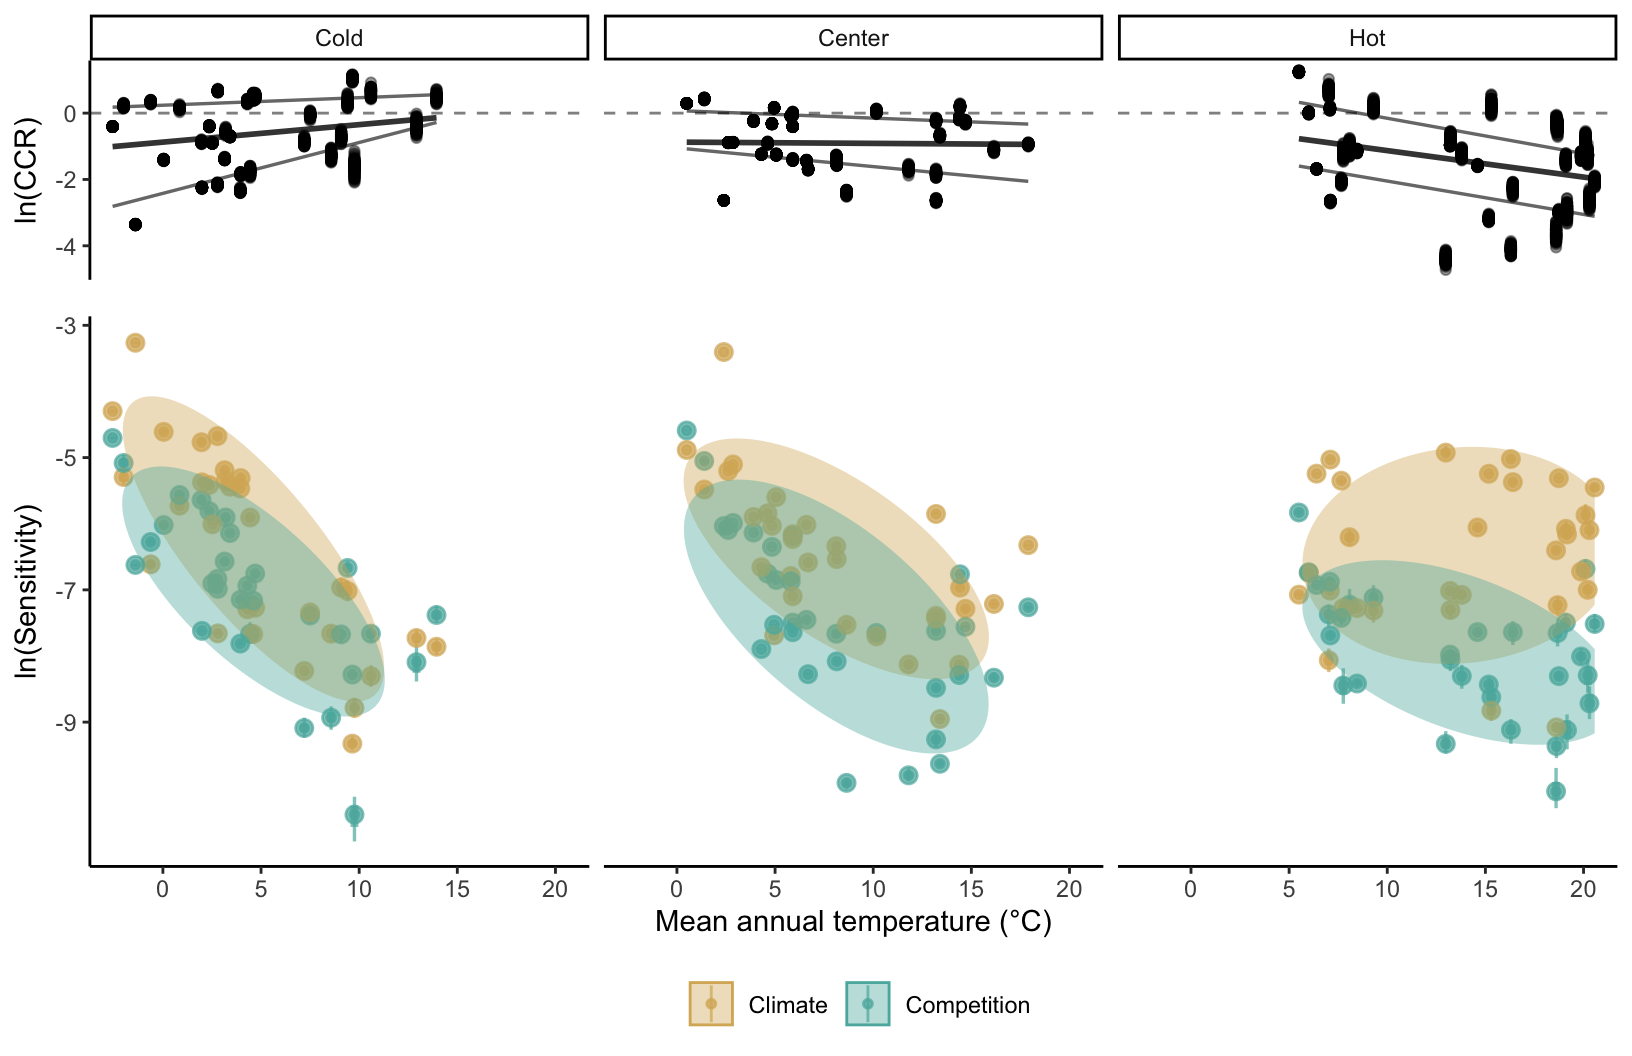
\includegraphics[width=1\textwidth,height=\textheight]{manuscript/figs/fig-sensBorder_temp-1.png}
\caption[{Bottom panels describe the sensitivity of species population
growth rate to competition (green) and climate (yellow) across the cold,
center, and hot temperature ranges.}]{Bottom panels describe the
sensitivity of species population growth rate to competition (green) and
climate (yellow) across the cold, center, and hot temperature ranges.
The top panels show the log ratio between competition and climate
sensitivities, where negative values mean climate sensitivity is
relatively higher than competition. We defined each species' temperature
range position as the median Mean Annual Temperature across all observed
plots for each cold, center, and hot range class. In the bottom panel,
species points are grouped by a Multivariate Normal Density function
with 75\% probability, while in the top panel, the lines represent the
25, 50, and 75\% quantile probabilities.}
\label{fig:temp_vs_comp}
\end{figure}
}

\hypertarget{discussion}{%
\section{Discussion}\label{discussion}}

We developed an integral projection model for 31 tree species linking
growth, survival, and recruitment to stand level \(\lambda\) in order to
assess the sensitivity of \(\lambda\) to climate and competition. Our
model advances previous analysis of tree species performance by (i)
explicitly incorporating climate and competition effects in the
recruitment model, (ii) distinguishing between conspecific and
heterospecific competition, while (iii) tracking model's uncertainty at
both the individual and plot levels. Moreover, we designed a modular
approach that is easily extendable to include any of the over 200
available species in the dataset and additional covariates influencing
each demographic rate.\\

The results reveal that, for all species, adding climate and competition
covariates enhances the predictability of all demographic components in
comparison to a simple random effect model without covariates.
Nevertheless, the most influential variable remained the local plot
conditions captured by the random effects. Therefore, we evaluated
species sensitivity to climate and competition while considering
plot-level variability. Across the species and their respective ranges,
we found that \(\lambda\) was more sensitive to temperature and
conspecific basal area of larger individuals. Furthermore, these
sensitivities were contingent on the range position of the species, with
climate being relatively more important than competition at both the
cold and hot range border. These findings contribute to a better
understanding of how tree species might respond to novel conditions
arising from climate change and perturbations, providing valuable
insights for their management.\\

\textbf{\emph{Fit of demographic components}}

Our model demonstrated remarkable coherence when reproducing the known
variation in traits related to growth, survival, and recruitment
components found in the literature. The intercepts for growth and
survival were correlated with maximal size and longevity
\citep{burns1990silvics}, while the recruitment intercept aligned well
with the seed mass \citep{diaz2022}. Additionally, the models
effectively reproduced the fast-slow continuum
\citep{SalgueroGomez2016}, showing a negative correlation between growth
and survival rate and a positive correlation between growth and
recruitment rate (Figure \ref{fig:figsupp8_ch2}). Regarding competition, the model captured
the negative correlation between density dependence and shade tolerance.
The model also matches a common expectation of communities where species
coexist, with a stronger response to conspecific competition relative to
heterospecific competition, crucial for biodiversity maintenance
\citep{Chesson2000a}. The intensity of conspecific density dependence
was also higher for fast-growing trees than for slow-growing ones
(Figure \ref{fig:figsupp9_ch2}), similar to observations in tropical trees \citep{Zhu2018}.
For climate, validation is challenging due to limited data on optimal
temperature and precipitation measures. Nevertheless, our results align
with others, indicating the presence of demographic compensation across
forest trees \citep{bohner2020, Yang2022}. Furthermore, the estimated
breadth of response to climate correlates with the range size (Figure
\ref{fig:figsupp10_ch2}), suggesting that the model captures information not explicitly
included.\\

Most of the variability in \(\lambda\) was associated with local plot
conditions captured by random effects, akin to previous studies
\citep{Vanderwel2016a, LeSquin2021}. This implies the influence of other
determinants of demography beyond climate and competition. For instance,
at a local scale, soil nitrogen content \citep{Ibanez2018} and mixed
mycorrhizal associations \citep{Luo2023} can enhance growth rates. At
larger scales, events such as wildfires and insect outbreaks play
crucial roles in forest dynamics and stand structure
\citep{Franklin2002}, causing synchronized mortality and altering stand
composition and abundance. While we focused on quantifying the effect of
climate and competition, other covariates may have greater importance in
driving variance in demographic rates. For instance, tree growth models
showed improved estimates when accounting for extreme climatic events
\citep{Sangines2017}, and unusual drought events, rather than average
precipitation, were the highest predictors of tree fecundity after
temperature \citep{Clark2011}.\\

\textbf{\emph{\(\lambda\) sensitivity to climate and competition}}

We found that the sensitivity of \(\lambda\) was higher for temperature,
followed by conspecific competition, across the species. Studies
examining the relative impacts of climate and competition on tree
performance yield diverse outcomes. For instance, while some suggest
that competition has a higher effect on growth than climate
\citep{GomezAparicio2011, LeSquin2021}, others find the opposite
\citep{CopenhaverParry2016}. Furthermore, the relative effect between
climate and competition can change between demographic components, where
growth is more sensitive to competition while fecundity to climate
\citep{Clark2011}. This disparity may arise from a tendency to evaluate
sensitivity to specific demographic rates rather than considering their
integrated effects. This is particularly critical since the population
growth rate does not respond equally to all covariates. We performed
additional sensitivity analyses, which revealed that most species are
primarily sensitive to recruitment, followed by survival, with a
relatively lower impact from growth (see Supplementary Material 3).\\

Assessing climate sensitivity across the species range distribution
revealed divergent responses. As species' performance changes
nonlinearly with climate, lower sensitivity values to a climate
covariate indicate that the species operates under optimal climate
conditions, whereas higher sensitivity values suggest the species is
deviating from its optimal climate condition. Overall, climate
sensitivity (primarily driven by MAT) was higher at both the cold and
hot range extremes. This implies that species coming from colder
temperatures exhibit optimal performance towards their warmer range, and
vice versa for species from hotter conditions. Interestingly, the
demographic components driving higher sensitivity to climate at the cold
and hot extremes differ. The recruitment and growth models primarily
influenced sensitivity at the cold border, while the survival model
dominated at the hot border (see Figure \ref{fig:figsupp11_ch2}). Previous studies have
indicated climate-constrained growth rates at the cold border for North
American \citep{Ettinger2013} and European \citep{Kunstler2021} trees.
Consistent with our results, a decrease in survival at the hot border
was observed for European trees \citep{Kunstler2021}, though not in
eastern North America \citep{Purves2009}.\\

The sensitivity of \(\lambda\) to competition increased almost linearly
toward colder temperatures for most species. Due to the nonlinearity
between species' performance and competition, the sensitivity of
\(\lambda\) to changes in competition decreases as stand density
increases (negative exponential shape). This implies that the observed
decrease in sensitivity to competition toward the hot range results from
an overall increase in stand density (i.e.~competition intensity).
Indeed, biotic interactions are often more critical at the warm range
border \citep{Paquette2021}. However, when evaluating only the growth
rate of North American \citep{Ettinger2013} and European
\citep{Kunstler2011a} trees, the effect of competition remains constant
across the climate range.\\

\textbf{\emph{Limitations and Future Perspectives}}

Structured population models, such as the IPM, play a crucial role in
capturing ontogenetic variability within tree population dynamics. While
the growth model inherently considers individual size, the survival and
recruitment models are size-independent. We attempted to incorporate the
widely assumed ``U-shape'' form of mortality rate changes with
individual size \citep{Lines2010}, but it performed worse than the
simple random effects one (Figure S6). Mortality has been observed to
increase with individual size \citep{Luo2011, Hember2017}, but its
significance appears to manifest only when interacting with climate and
competition \citep{LeSquin2021}. The challenge in capturing size
dependence in the survival model likely stems from the lack of
information on small individuals (dbh \textless{} 12.7 cm) and the
rarity of larger individuals in datasets, even for extensive forest
inventories \citep{Canham2017}. Despite not explicitly including
individual size in the survival model, its indirect influence is
included with the asymmetric competition, where smaller individuals
experience higher competitive pressure. Another limitation of this
model, shared with many models using forest inventory data
\citep[Kunstler2021;][]{LeSquin2021, Guyennon2023}, is its focus on
adults, while tree fecundity can be influenced by climate
\citep{Clark2021}, and the dynamics of recruitment may not necessarily
align with those of adults
\citetext{\citealp{SerraDiaz2016}; \citealp{Wason2017}; \citealp[but
see][]{Canham2016}}.\\

The modular nature of our approach makes it easily extensible to include
new species or covariates. For instance, additional covariates such as
water balance or evapotranspiration could be tested to evaluate the
impact of drought-induced mortality \citep{Peng2011}. Furthermore,
exploring the interaction between climate, competition, and individual
size can enhance predictions of demographic rates
\citep{Peng2011, Ford2017, Rollinson2016, LeSquin2021}. An overlooked
but computationally expensive improvement involves jointly fitting the
growth, survival, and recruitment models. This would enable leveraging
ecological knowledge, such as life history tradeoffs, by sharing
information between processes with abundant data (e.g.~growth) and those
with scarce data (e.g.~recruitment). Future steps should focus on better
understanding the variability captured by random effects and translating
it into ecological processes. While we addressed individual and
plot-level model uncertainty, further considerations for other sources
of variability arising from temporal stochasticity in climate and
competition covariates are essential. This will enhance our
understanding of the effects of spatiotemporal variability on species
performance across their range \citep{Holt2022}.\\

\singlespacing
{\renewcommand{\bibname}{References}
\renewcommand{\bibsection}{\section{\bibname}}
\bibliography{chapter2/manuscript/references}}
\bibliographystyle{styles/myBEAS}
